\documentclass[10pt,a4paper]{article}
\usepackage[latin1]{inputenc}
\usepackage{amsmath}
\usepackage{amsfonts}
\usepackage{amssymb}
\usepackage{graphicx}

\usepackage[left=1.00in, right=1.00in, top=1.10in, bottom=1.00in]{geometry}
\author{Michael Reed}
\title{Mathematics of India Preceding the Modern Era}
\date{Revision 1.5, 2016}
\begin{document}
\maketitle

\begin{abstract}
Various mathematical subjects of Indian texts predating the modern era are described as well as the philosophical role and functioning of mathematics in Indian culture.
\end{abstract}

%\begin{itemize}
%\item sankhyana = enumeration
%\item ganita = science of calculation
%\item triprasna = direction, place, time
%\item shastra = work of scripture, collection of procedures / sutras
%\item sutra = a rule or aphorism in Sanskrit literature, or a set of these on a technical subject
%\item upapatti = proof
%\item paradha = highest number
%\item sunya = zero, void
%\item purna = infinity, complete, full
%\item lopa = null morpheme, Panini's Astadhyayi
%\item abhava = absence, non-existence (Buddha and Naiyayika philosophers)
%\item samagarbha = magic square
%\item tarka = proof by contradiction?
%\end{itemize}

\section{Shastras \& Sutras}

Broadly speaking, the mathematics of India can be split into four eras: ancient, classical, medieval, and modern. In this time, the Indians developed geometrical transformations using lines, shapes, and figures that they described in their texts. Mathematical ideas from Buddha  and Jaina regarding infinity, logarithm, zero, and decimals ended up contributing to mathematics and astronomy in Indian culture. 

A sutra is a rule or aphorism in Sanskrit literature while shastras are works of scripture being collections of sutras and procedures. In this way the concepts of sankhyana (enumeration) and ganita, which is the science of calculation and computation, were passed down to explain triprasna--the three important topics in astronomy dealing with direction, place, and time.

Panini deeply influenced Indian mathematical texts and sutras and is culturally equivalent to Euclid, as he dealt with derivation of grammars and logical reasoning using recursive generative conventions governing rule application and interaction; an early precursor to computer science.

%\begin{figure}[h]
%\centering
%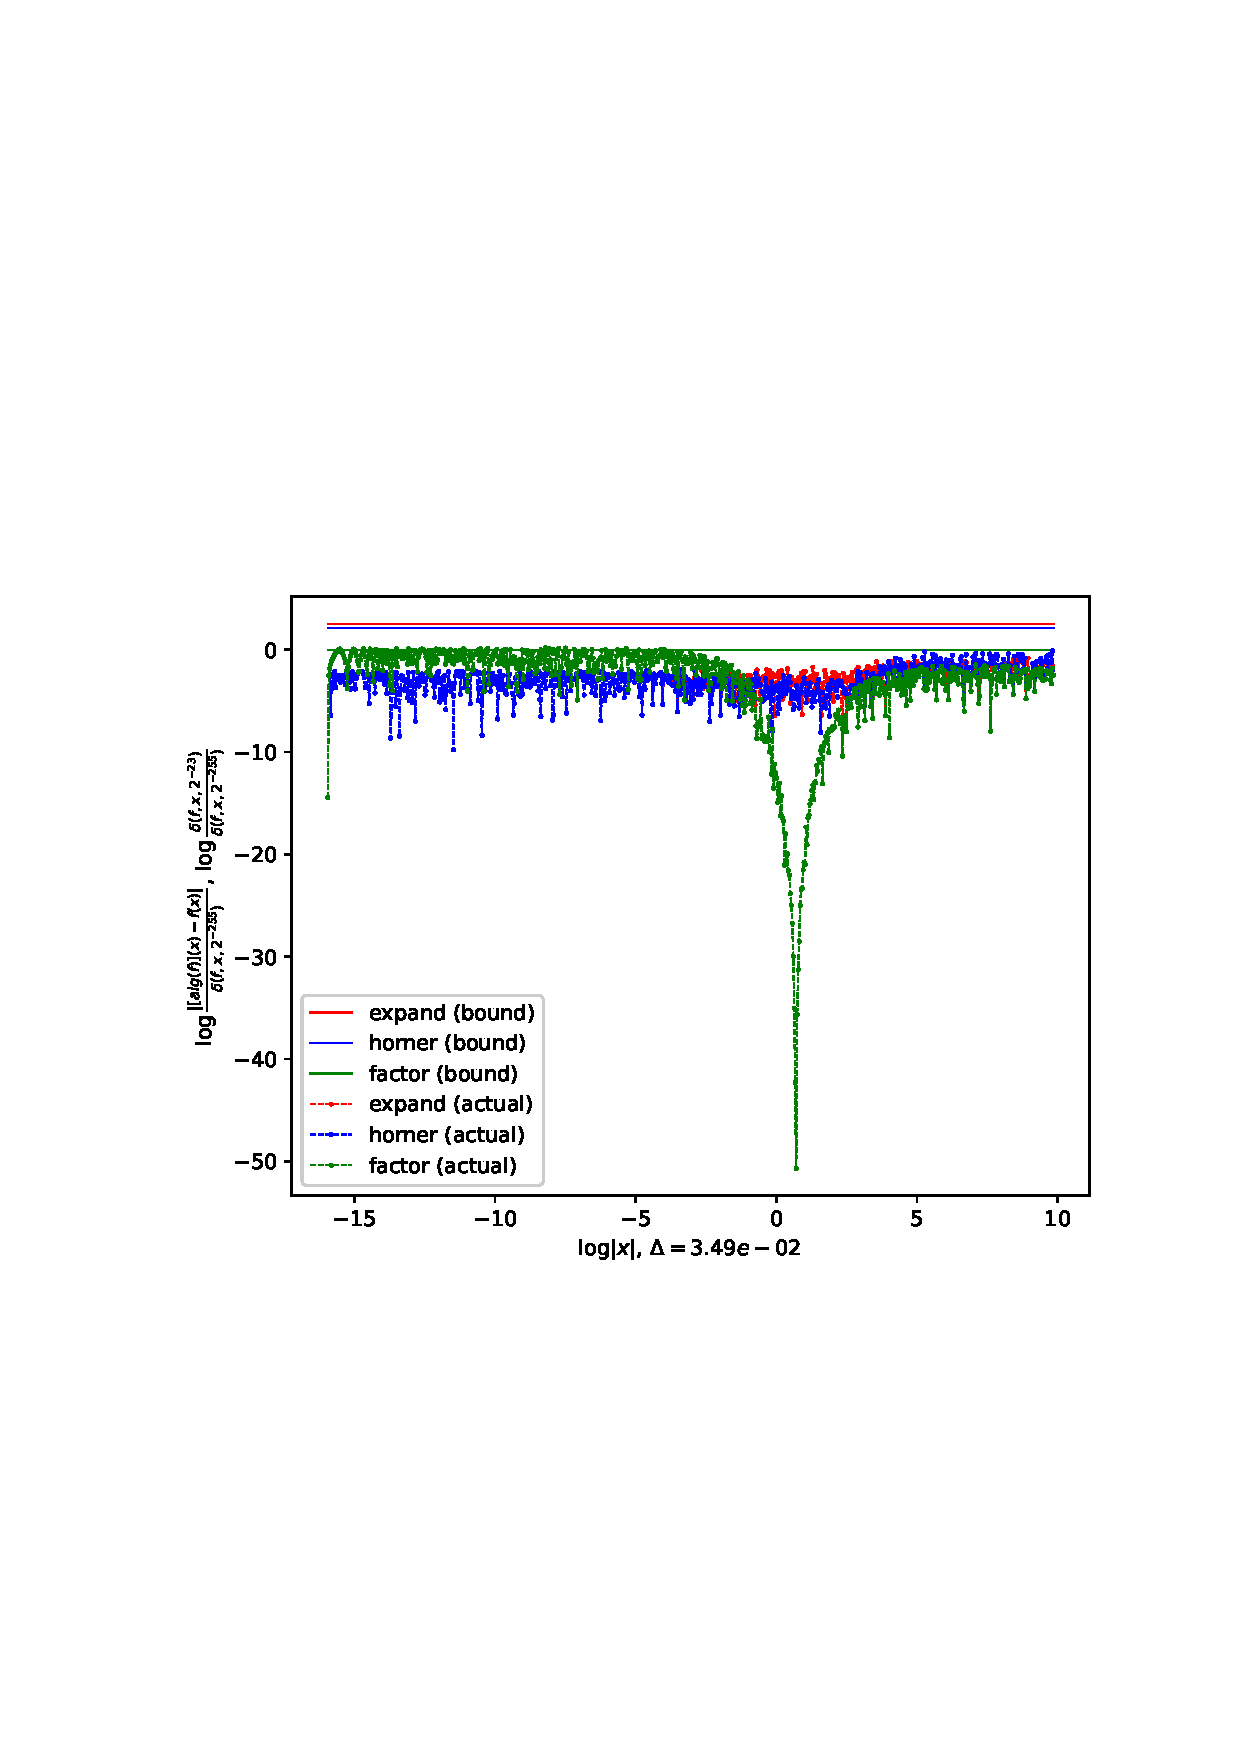
\includegraphics[width=0.8\linewidth]{2.png}
%\end{figure}

\section{Decimal Place Value System}
Today's decimal place value system that is widespread in modern mathematics was developed by Indian mathematicians along with representation for the null quantity. The decimal number quantity $N_b$ with $\alpha+\beta$ digits $d_k$ before ($\alpha$) and after ($\beta$) the decimal separator ($\sigma$) is an algebraic concept based on a polynomial series in base $b=10$, stated in modern symbolic notation by
\begin{equation}
N_b = \sum_{k=-\beta}^{\alpha-1} d_k b^k = d_{\alpha-1}b^{\alpha-1} + \cdots + d_{k+1}b^{k+1} + d_{k}b^{k} + d_{k-1}b^{k-1} + \cdots + d_{-\beta} b^{-\beta},
\end{equation}
which is compactly written by successively placing all the digits into a row as
\begin{equation}
N_b = d_{\alpha-1} \cdots d_{k+1} d_k d_{k-1} \cdots d_0 \sigma d_{-1} \cdots d_{-\beta}
\end{equation}
with a decimal point separator $\sigma \rightarrow .$ after $k=0$ to indicate fractional quantities if $\beta > 0$.

During the Vedic period of Indian religious texts, names for decimal quantities existed for large values up to parardha or $10^{12}$. Before the numeral symbols were devised, decimal quantities were referred to verbally using code words. The Upanishads speak of sunya ($0$) and purna ($\infty$). With Panini's work Astadhyayi, the concept lopa of the zero-morpheme becomes a fundamental part of Indian linguistic culture. Philosophers of Buddha and Jaina traditions discuss concepts of non-existence / absence using sunya and abhava. Scholars such as Pingala used zero as a marker by rupe sunyam. During (c. 50 CE) philosophers of the Vasumitra and Vasabhasya discuss the changing connotation of the same symbol in a place value system in analogy with a woman changing in relation to others from daughter to mother and so forth. Commentaries on Indian mathematics sometimes discussed special techniques of calculation that are founded in the algebraic formalism of the place value system, such as the vajrabhyasa (vertical and crosswise multiplication technique). Indian mathematics was practically powerful and spread to many other cultures such as Syria, Cambodia, and Islam due to its usefulness to everyone who used it, including traders and architects. From there, the spread of the decimal place value system continued into Europe and the rest of the world by the works of authors such as al-Khwarizmi and Fibonacci.

%al-Khwarizmi (825), Hisab al Hindi introduced Indian math to west

%Sphujidhvaja, earliest dated use of decimal system in Greek astrological translation
\newpage

\section{Continued Fractions}
An alternative to representing a numerical value as a decimal series expansion is to write it as a sequence of values $q_k \in\mathbb{Z} $ defined from a continued fraction expansion (CFE),
\begin{equation}
q_0 + \underset{k=1}{\overset{n}{\rm K}} ~\frac{1}{q_k} \triangleq q_0 + \cfrac{1}{q_1 + \cfrac{1}{q_2 + \cfrac{1}{\ddots \cfrac{\ddots}{q_{n-1}+\cfrac{1}{q_n}}}}},
\end{equation}
here expressed using Gauss' continued fraction operator $\rm K$. Kettenbruch is compactly represented by
\begin{equation}
[ q_0; q_1,q_2,q_3,\ldots, q_k, \ldots ].
\end{equation}

As with decimal series expansions, these continued fractions can be both finite and infinite sequences. When an infinite CFE with $n=\infty$ is truncated, the resulting quantity $r_0/r_1\in\mathbb{Q}$ is always the best possible rational approximation up to the $n$th order of the irrational quantity. Unlike the decimals, one primary difference is that CFEs are independent of their numeral base $b$. An $n$th order partial fraction can produce a decimal series with more than $n$ terms, making it a more compact representation.

\section{Algebra \& Geometry}
Baudhayana in the 8th century BCE gave lists Pythagorean triples along with a statement of the Pythagorean theorem, also giving the approximate value of $\sqrt{2}$ as the $7$th order CFE convergent
\begin{equation}
\sqrt{2} = [1;2,2,\dots] \approx 1 + \frac{1}{3} + \frac{1}{3 \cdot 4} + \frac{1}{3 \cdot 4 \cdot 34} = \frac{577}{408} = [1;2,2,2,2,2,2,2] = 1.414215686\dots
\end{equation}

Pingala was working with binary combinatorics in the 3rd century BCE to enumerate grammatical rule combinations and was aware of the combinatorial identity.
%In (c. 629), Bhaskara I gave a method for squaring numbers in $n(n-1)/2$ multiplication steps for an $n$ digit number. 
%Aryabhatiyabhasya, Mahabhaskariya, simple formula for sine function (ratio of 2 polynomials)
%\begin{figure}[h]
%\centering
%\includegraphics[width=0.5\linewidth]{18.png}
%\end{figure}
In the Sanskrit text Katyayana Sulvasutra of the 3rd century BCE, a generalized Pythagorean theorem for the problem of finding a square that is $n$ times that of a given square $a^2$ is given, which can today be symbolically expressed as
\begin{equation}
\alpha^2 - \beta^2 = \gamma^2 = na^2 = \left[ \frac{(n+1)a}{2} \right]^2 - \left[ \frac{(n-1)a}{2} \right]^2.
\end{equation}

During the 6th century, the Indian astronomer mathematician Varahamihira improved the accuracy of sine tables to 4 decimal place values and also discovered the trigonometric identities
\begin{align}
\sin^2(x)+\cos^2(x)&=1, & \sin(x)&=\cos\left(\frac{\pi}{2}-x\right),  & &\qquad\text{and}\qquad & 1-\cos(2x)&=2\sin^2(x).
\end{align}
Later in the 7th century, Brahmagupta had devised a method to interpolate new values at $a+xh$ from tabulated sine data of interval $h$ using a second-order Newton-Stirling forward difference method \cite{srinivas-calculus},
\begin{equation}
f(a+xh) \approx f(a) + x \left(\frac{f(a+h)-f(a-h)}{2}\right)+\frac{x^2 (f(a)-f(a-h))^2}{2!}.
\end{equation}
Jain mathematician Mahavira wrote a book called Ganita Saar Sangraha in the 9th century on numerical mathematics and the science of calculation. He had a formula approximating the area and perimeter of ellipses. In numerical problems for geometry, he usually gave two rules: one for rough calculation and the other for more accurate results. Like many other mathematicians of India, he gave problems that lead to indeterminate linear equations of up to four variables.%, such as$\{p+x=2(y+z), p+y=3(x+z), p+z=5(x+y) \}$ with the smallest positive integer solution $\{p=15,x=1,y=3,z=5\}$.

%\subsection{Aryabhatiya Ganitapada}


Verses from the Aryabhatiya Ganitapada \cite{ref:aryabhatiya} cover diverse topics including samkhyasthana (place values), vargaparikarma (squaring), ghanaparikarma (cubing), vargamulanayana (square-root), ghanamulanayana (cube-root), area of triangle, volume of regular tetrahedron, area of circle, volume of sphere, area of trapezium, approximation of $\pi$, jyanayana (computing sine), karnanayana (Pythagorean theorem), saranayana (intercepted arcs), sredhi-ganita (repeated summation), mulaphalanayana (interest and principal), bhinna-purikarma (fractional arithmetic), pratiloma-karana (inverse processes), yogakolanayana (meeting time of two bodies), and kuttakara-ganita (indeterminate equations). Aryabhata goes on by describing details of measuring time, astronomical cycles, and spherical geometry.

%Aryabhata I, uses decimal place value system, ?spherical geometry and astronomy?

\newpage

\subsection{Cyclic Quadrilaterals}
In (c. 628) Brahmagupta gave the formula for the area $A_c$ of any cyclic quadrilateral with the side lengths of $L=\{a,b,c,d\}$, where $L\subset\mathbb{R}$, having a semiperimeter $s \leftarrow (a+b+c+d)/2$. Such convex quadrilaterals can be inscribed in a circle of radius $r_c$ and have the property that
\begin{equation}
\alpha+\gamma=\beta+\delta=\pi,
\end{equation}
meaning that the sums of the opposite angles are equal to the ratio of a circle's circumference to the diameter. The cyclic quadrilateral area formula of Brahmagupta,
\begin{equation}
A_c=\sqrt{(s-a)(s-b)(s-c)(s-d)},
\end{equation}
is a generalization of Heron's triangle area formulation by the fact that a triangle is merely a quadrilateral with one length equal to zero. 
During the 15th century, Parameshvara \cite{ref:Parameshavra} gave the circumradius $r_c$ of the cyclic quadrilateral as
\begin{equation}
r_c=(4A_c)^{-1}\sqrt{(ab+cd)(ac+bd)(ad+bc)}.
\end{equation}
Additionally, the length of the diagonals $e$ and $f$ were given in terms of $L$ by Brahmagupta \cite{ref:Brahmagupta} as
\begin{align}
e&=\sqrt{\frac{ad+bc}{ab+cd}(ac+bd)}, & f&=\sqrt{\frac{ab+cd}{ad+bc}(ac+bd)}, &\qquad\text{or}\qquad \frac{f}{e}&=\frac{ab+cd}{ad+bc}.
\end{align}
Going into the 20th century, Coolidge \cite{ref:Coolidge} showed how it is possible to obtain the area $A_g$ of a general convex quadrilateral in terms of the length of its sides $L$ and diagonals $\{p,q\}$ using
\begin{equation}
A_g=\sqrt{(ab+cd)(ac+bd)(ad+bc)-(ac+bd+pq)(ac+bd-pq)/4}.
\end{equation}
It can be seen that Brahmagupta's formula $A_c$ is the special case of $A_g$ satisfying Ptolemy's theorem,
\begin{equation}
pq\implies ef=ac+bd,
\end{equation}
after applying it as a substitution.


\section{Indeterminate Polynomials}
During the 6th century, Aryabhata first demonstrated the use of continued fraction expansions to solve linear equations using Kuttaka. In any finite continued fraction, the sequence $\{q_k\}$ is equivalent to the Euclidian division principle $r_{k+1}=r_{k-1}-q_k r_{k}$ used to calculate Bezout's identity $r_0 x + r_1 y = \gcd(r_0,r_1)$.
\begin{equation}
\left\{ 
%\frac{a_n}{b_n} = q_0 + \frac{r_0}{b_n} , \frac{b_n}{r_0} = q_1 + \frac{r_1}{r_0} , 
\frac{r_0}{r_1} = q_0 + \frac{r_2}{r_1} ,\dots, \frac{r_{k}}{r_{k+1}} = q_k + \frac{r_{k+2}}{r_{k+1}} ,\dots, \frac{r_{n}}{r_{n+1}} = q_n \right\}.
\end{equation}
In order to obtain the base values $\{\sigma_k,\tau_k\}\in\{x,y\}$, Kuttaka is used to obtain values from corresponding sequences $\sigma_{k+1}=\sigma_{k-1}-q_k \sigma_{k}$ and $\tau_{k+1}=\tau_{k-1}-q_k \tau_{k}$ using the starting values $\sigma_0=1$, $\sigma_1=0$, $\tau_0=0$, and $\tau_1=1$. When $r_{k+1}=0$, the property $\gcd(r_0,r_1)=r_k=r_0 \sigma_k + r_1 \tau_k$ holds.

For $a=r_0$ and $b=r_1$, Brahmagupta \cite{ref:brahmagupta-textbook} was the first to show all the possible solutions $S\subset\mathbb{Z}=\{x,y\}$ for the indeterminate linear equation
\begin{equation}
c=ax+by=d(sx+ty) \Leftrightarrow d|c,
\label{eq:ipeq}
\end{equation}
where $d=\gcd(a,b)=r_k$ and $\{a,b,c,d\}\subset\mathbb{Z}$. 
Since $a=d s$ and $b=d t$, it is known that $s$ and $t$ are relatively prime, satisfying the relationship
\begin{equation}
\gcd(s,t)=\gcd\left( \frac{a}{d},\frac{b}{d} \right) = 1.
\end{equation}
If $\{x_i,y_i\}=S_i\in S$, then using $S_0$ and $S_i$ in equation~(\ref{eq:ipeq}) leads to
\begin{align}
ax_0+by_0&=c=ax_i+by_i & &\qquad\text{and}\qquad & a(x_i-x_0)&=b(y_i-y_0).
\label{eq:ipp}
\end{align}
Eliminating $d$ by substituting $a$ and $b$ in equation~(\ref{eq:ipp}) and using Euclid's lemma leads to the fact that
\begin{equation}
s|t(y_i-y_0)=s|t s i \Leftrightarrow t|s t i=t|s(x_i-x_0).
\end{equation}
As a result, all the other possible solutions $S_i$ are obtained using
\begin{align}
x_i&=x_0+t i=x_0+\frac{b}{d}i, & y_i&=y_0+s i=y_0+\frac{a}{d}i
\end{align}
for any value $i\in\mathbb{Z}$, given a particular base solution $S_0=\{\sigma_k,\tau_k\}$ obtained from Kuttaka.

\newpage

Indian mathematicians also had great interest in what is today falsely named the Pell equation. Brahmagupta worked on solutions to this equation, which was later generalized by Jayadeva and refined by Bhaskara II. Using the Chakravala method, an integral solution in $S\subset\mathbb{Z}=\{x,y,\lambda\}$ can be obtained and recomposed \cite{chakravala-srinivas} into another solution $S_{i+1}\in S$ of increasing size for the general Bhaskara equation
\begin{equation}
x^2-\zeta y^2=\lambda,
\end{equation}
where $\zeta\in\mathbb{Z}$ and $\sqrt{\zeta}\notin\mathbb{Z}$. Brahmagupta's identity says that for the solutions $S_a$ and $S_b$ it is known that
\begin{equation}
\{x_ax_b\pm \zeta y_ay_b,x_ay_b\pm x_by_a,\lambda_a \lambda_b\}\in S,
\end{equation}
otherwise known as Brahmagupta's bhavana \cite{ref:video} or principle of composition. In consequence, for any $S_i$
\begin{equation}
\left(\frac{x_i^2+\zeta y_i^2}{\lambda_i}\right)^2-\zeta\left( \frac{2x_i y_i}{\lambda_i}\right)^2=1
\end{equation}
or, for Pell's equation, when $\lambda = 1$ it follows that there is a recurrence relation
\begin{equation}
\{x_i^2+\zeta y_i^2,2x_i y_i,1\}\in S \Rightarrow \{x_{i+1},y_{i+1},1\} = S_{i+1} ,
\end{equation}
from which infinite solutions $S_{i+1}$ can be obtained. Thus it is possible to repeatedly apply Brahmagupta's identity using a base solution $S_0$. Swamy \cite{ref:brahmagupta-theorem} shows that this can be rewritten as a generalized polynomial equivalent to a Chebyshev polynomial of the first and second kind. Using $S_0=\{1,0,1\}$ and $B_0=0$ to obtain $S_{n+1}$ in the general Chakravala algorithm based on Bhaskara's lemma, $S_n$ is composed with $S_B = \{B_{n+1},1,B_{n+1}^2-\zeta\}\in S$ using bhavana $\forall B_{n+1} \in \mathbb{Z} : \underset{B_{n+1}}{\operatorname{argmin}} |B_{n+1}^2 - \zeta| \equiv - B_{n}(\!\!\!\mod{\lambda_n})$, such that
\begin{equation}
S_{n+1}=  \left\{ \frac{x_n B_{n+1} + \zeta y_n }{|\lambda_n|}, \frac{x_n + y_n B_{n+1} }{|\lambda_n|}, \frac{B_{n+1}^2 - \zeta}{\lambda_n} \right\}.
\end{equation}

The algorithm is repeated until a $\lambda_{n+1}=1$ is obtained and has been proven to always terminate with a solution $S_i$ by Lagrange in (c. 1768) \cite{bauval}. If $\lambda_{n+1}=\pm1\vee\pm2\vee\pm4$, then the bhavana principle can be applied to obtain infinite solutions $S_{i+1}$ as shown by Brahmagupta. For example, a particular case is
\begin{equation}
1766319049^2-61\times 226153980^2=1 .
\end{equation}
Notably, the $\zeta=61$ case was issued as a challenge by Fermat to Frenicle in (c.~1647) and was later solved by Euler in (c. 1732), while Bhaskara II used this case as an example many centuries earlier (c. 1150) to approximate $\sqrt{\zeta}\notin\mathbb{Q}$ using rational solutions. 
The quotient result is equivalent to the partial CFE evaluated with 21 terms but obtained in less steps. 
This case has an accuracy of 17 decimal places. 
\begin{equation}
\sqrt{\zeta} \approx \frac{x_i}{y_i} \Rightarrow \sqrt{61} = \left[ 7;\overline{1,4,3,1,2,2,1,3,4,1,14} \right] \approx \frac{1766319049}{226153980}=7.81024967590665439...
\end{equation}

%Narayana's folding method for samagarbha (magic square)

\section{Infinite Series}
Madhava (c. 1350) calculated the circumference $C$ of a circle with radius $r$ using the Leibniz series,
\begin{equation}
C = 8r \frac{\pi}{4} = 8r \arctan (1) = 8r \lim\limits_{n\rightarrow\infty} C_L(n) = 8r \lim\limits_{n\rightarrow\infty} \left( \sum_{k=0}^{n} \frac{(-1)^k}{2k+1} \right),
\end{equation}
a series with sublinear convergence, requiring 5 billion terms for 10 decimals of accuracy. In order to speed up the convergence, Madhava gave special error correction terms $e_i(n)$ added to the series as
\begin{equation}
C \approx C_M (n,r) = 8r \left(C_L(n) + e_i (n+1)\right)
\end{equation}
and offers a choice of different orders of accuracy for the error term \cite{srinivas-calculus} with
\begin{align}
e_1 (n) &= \frac{(-1)^{n}}{4n}, & e_2 (n) &= \frac{n(-1)^{n}}{4n^2+1}, & e_3 (n) &= \frac{(n^2+1)(-1)^{n}}{n(4n^2+5)}.
\end{align}
Using this method, Madhava gives the value of $\pi$ to 11 decimal place accuracy with $n=50$ terms. 

Alternatively, Madhava also has given an even more rapidly converging method using the formula
\begin{equation}
\pi = \sqrt{12} \sum_{k=0}^{\infty} \frac{(-3)^{-k}}{2k+1},
\end{equation}
with which the first 11 decimal digits can be correctly obtained using the first 21 terms.

Another notable Indian mathematician centuries later named Ramanujan gave an exact formula that was used to make an estimate for the value of $\pi$ with 17 million digits of accuracy, as
\begin{equation}
\frac{1}{\pi} = \frac{2\sqrt{2}}{9801} \sum_{k=0}^{\infty} \frac{(4k)!(1103+26390k)}{(k!)^4 396^{4k}}
\end{equation}
gives an additional 8 decimals of accurate digits per term.

While lacking the modern factorial symbolism, the Kerala astronomers \cite{ref:series} between the 14th and 16th centuries dealt with calculus concepts like Taylor-Maclaurin series and had numerous infinite series expressions for evaluating trigonometric quantities in the Tantrasangrahavakhya, such as
\begin{equation}
\arctan \left( \frac{y}{x} \right) = \sum_{k=0}^{\infty} \frac{(-1)^k}{(2k+1)} \frac{y^{2k+1}}{x^{2k+1}},
\end{equation}
\begin{equation}
\sin \left( \frac{x}{r} \right) = \sum_{n=0}^{\infty} x (-1)^n \prod_{k=1}^{n} \frac{x^2}{r^2 ((2k+1)^2+2k)},
\end{equation}
\begin{equation}
r \left( 1- \cos \left( \frac{x}{r} \right) \right) = \sum_{n=1}^{\infty} r (-1)^{n+1} \prod_{k=1}^{n} \frac{x^2}{r^2 ((2k+1)^2+2k)}.
\end{equation}
%Madhava (1350), founder of Kerala School, infinite series ($\pi$, sine and cosine, fast convergence)

The Kerala astronomers also worked with the geometric series $g(x)$ having the sum of
\begin{equation}
g(x)=\sum_{k=0}^{\infty}x^k =\frac{1}{1-x} \iff |x|<1,
\end{equation}
resulting in converging partial sums. However, the mathematician Ramanujan also worked with divergent series and investigated the meaning of results such as Grandi's series $g(-1)$, which can be validly interpreted if the summation definition is extended to the Cesaro convergent of averaged partial sums,
\begin{equation}
g(-1)=1+1-1+1-1+\dots \triangleq \lim\limits_{n\rightarrow\infty}n^{-1}\sum_{k=1}^{n}\sum_{j=0}^k (-1)^j = \frac{1}{2}.
\end{equation}
In the  development of complex analysis it has been shown that there are a multiplicity of methods for summing an infinite series by analytic continuation, such as the Ramanujan summation formula
\begin{equation}
\sum_{k=1}^x f(k) = C + \int_0^x \! f(t) \, \mathrm{d} t + \frac{1}{2} f(x) + \sum_{k=1}^\infty \frac{B_{2k}}{(2k)!} f^{(2k-1)} (x),
\end{equation}
which is related to the Euler-MacLaurin formula in consideration with the Bernoulli numbers. 
Using these extended methods, it is possible to attain finite values for problems that are logically contradictory or impossible using traditional calculus rules. %Mathematicians such as Euler and Ramanujan were not constrained in the same sense of thinking as those following Hilbert's program or the Greek approach, who were nevertheless transcended by ones such as G�del or Turing. 

Another function related to the geometric series studied by Ramanujan is the Riemann zeta function
\begin{equation}
\zeta(s) = \sum_{k=1}^{\infty}k^{-s} = 2^s \pi^{s-1} \sin\left(\frac{\pi s}{2} \right) \Gamma(1-s)\zeta(1-s),
\end{equation}
whose functional equation was also discovered by him. Thus, it is possible to know that $\zeta(-1)=-12^{-1}$.
\begin{equation}
\sum_{k=1}^{\infty} \frac{k^{13}}{e^{2\pi k}-1} = \frac{1}{24}
\label{eq:pec}
\end{equation}
Ramanujan left behind peculiar sums (\ref{eq:pec}). 
In his paper \textit{On certain arithmetical functions}, Ramanujan defined the $\tau$-function and made multiple conjectures regarding it using a numerical tabulation up to $n=30$. This work was later extended for further modular forms by Mordell, Hecke, and Deligne \cite{gamelin,ref:summingitup}.
\begin{equation}
\Delta(z) = q \prod_{n\geq 1} (1-q^n)^{24} = \sum_{n\geq 1} \tau(n) q^n = \frac{E_4^3 - E_6^2}{1728} = \eta(z)^{24}
\end{equation}

%In modern transcendental number theory, concepts of mathematicians from India in the past are utilized to compute values such as the Riemann-Pad� function.

\newpage

\section{Mathematical Philosophy}
%\section{Astronomy}
The purpose of Indian mathematics was often revolving around making calculations in astronomy. In (c.~1500), Nilakantha Somayaji gave a revised planetary model based on the heliocentric idea due to observations of Mercury and Venus revolving around the Sun inside Earth's orbit. Various mathematicians from other cultures sometimes interacted and exchanged knowledge with the Indian mathematicians. Jyesthadeva in (c. 1530) gave a systematic exposition of mathematics and astronomy using proofs.

%Sawai Jayasimha (1700), mathematics, astronomy, translation from persian Euclid and Ptolemy

%Acyuta Pisarati (c. 1600), Putamana Somayaji (c. 1700), and Sankaravarman (c. 1830)  were some of the later Kerala astronomers.

%Candrasekhara Samanta (1869), Orissa, all three lunar inequalities
%\item upapatti = proof
Commentaries and expositions play an important role in passing down and developing knowledge that was previously transmitted orally in the Sanskrit tradition. 
Importance of upapattis (proofs) is emphasized by Bhaskara II. %, explains the role of proof in mathematics, etc
In Indian mathematics, the main purpose of proof was to improve the mathematical community. Without knowledge of the upapattis an Indian mathematician could not be sure of his understanding and be free of doubt. Thus, according to Ganesa Daivajna, the purposes of upappattis are to remove confusion and doubts regarding the validity and interpretation of mathematical results and procedures as well as to obtain respect in the community of mathematicians. However, much of the mathematical tradition was informal and passed down verbally, with discoveries based on recursive logical rule systems and intuitive use of mathematical induction. 

Indian mathematicians adhere to the constructivist mathematical philosophy and therefore don't emphasize proof by contradiction \cite{ref:video}, as they don't necessarily believe that a formal mathematical system can be entirely consistent in the same sense as the theorem of incompleteness \cite{ref:incompleteness} says. This is demonstrated by the fact that they did not set up an axiomatic system because they did not believe all necessary assumptions can be stated. They also did not heavily rely on arguments like reductio ad absurdum, yet nevertheless they arrived at new results and discoveries throughout their history and extended their mathematics.

Multiplicity of viewpoints is what the Jain philosophers called anekantavada. Their non-one-sidedness implies that nondualisms are ubiquitous and that statements can be both true and false at the same time, otherwise a logical contradiction. This perspective is also called dialetheism or Catuskoti by the Buddhists as an attempt to resolve some paradoxes of self-contradictory statements. It is evident that mathematicians of India, such as Ramanujan, must have been influenced by these ancient philosophies when making sense of divergent infinite series with logic defying contradictory partial sums.
%\begin{equation}
%\{ P , \neg P, P \land \neg P, \neg(P \lor \neg P) \}
%\end{equation}

%Mahaviracarya (850), importance of ganita, Ganitasarasangraha

%Bhaskaracarya II (1150), Upapattis (proofs) in Vasanabhasyas

%Jyesthadeva (1530), systematic exposition of math and astronomy using proofs, Yuktibhasa has calculus, commentaries by Sankara Variyar (1540)

%Jnanaraja (1500), Ganesa Daivajna (1507), Suryadasa (1541), Krsna Daivajna (1600), commentaries with upaattis

%\subsection{Additional People}
%\begin{itemize}
%\item Varahamihira (505)
%\item Brahmagupta, mathematics of zero and negative numbers, algebra
%\item Baksali manuscript
%\item Sridhara, Lalla (750), Govindasvamin (800)
%\item Prthudakasvamin (860), Munjala (932), Aryabhata II (950), Sripati (1039), Jayadeva (1050)
%\item Thakkura Pheru, (1300), Rajaditya, Pavuluri Mallana (1350) in Telugu
%\item Narayana Pandita (1350)
%\item Paramesvara (1400)
%\item Munisvara (1603), Kamalakara (1616)
%\end{itemize}

%\section{Inflection \& The Modern Era}
%\newpage
	\bibliography{Mathematics-India}
	\bibliographystyle{plain}

\end{document}
